\section{Machine Learning for Classification}
\label{sec:org837d169}
The main goal Machine Learning is set to achieve, is the development of algorythms equiped with the capabillity of learning from data automatically. In particular, an artificially intelligent system must have the ability to identify objects in its surroundings, as well as anticipate the actions of its environment, in order to make informed decisions. Due to this, machine learning techniques tend to be more oriented towards forecasting, rather than prediction.
\subsection{Decision trees and Supervised Learning}
\label{sec:org9e96dfd}
The distinction between different particles, can be regarded as a classification problem where the target, is the prediction of a categorical output variable(i.e. lepton, boson), based on one or more input variables(i.e momenta components). Classification problems in  machine learning can be solved with supervised learning. In such procedure, a training data set is being used for the development(training) of a model that is able to perform the classification task. The output of the model is then beeing tested and evaluated on previously unseen data.

Before presenting any specific method of solving classification problems It is important to present an overview of the key elements in supervised learning.

\subsubsection{Supervised learning}
\label{sec:orgc2bcda3}
Let us pose the following problem:
Given a data set \(D= (\vec{X}, \vec{y})\), where \(\vec{X}\) is a matrix of the independet variables and \(\vec{y}\) is a vector of dependent variables, we want to find a model \(f(\vec{x} ; \vec{\theta})\),  that can predict an output from a set of input variables. Moreover, we  want to be able to judge the performance of the model on a given data set. To do that we need to define a cost function \(C(\vec{y}, f(\vec{X}; \vec{\theta}))\), such that the model will have to find the parameters \(\theta\) that minimize the cost function.\cite{Mehta_2019}

This the mathimatical pustulation of a supervised learning problem. I will now, in brief, discuss the role and interpretation of each of the 'ingredients' stated above.

\begin{itemize}
\item Model
\label{sec:org31e7a41}

The model, is a mathematical function \(f\text{ : } \vec{x} \rightarrow y\) of the parameters \(\theta\). Given a set of parameters, the output of the function, the prediction \(y_{i}\), is derived from the input variables \(\vec{x}\).
The parameters are undefined. The task of the training is to estimate the set of parameters from the training data set.
In a classification problem(something is of type a or it is not), it is possible to use the logistic transformation of the function output, to obtain the probability of the positive class.

\item Cost function
\label{sec:orgac31e22}

The cost function, also known as an objective function, is represented by mathematical function and it measures how well a model fits the training data. The cost function is used to train the model by finding the best set of parameters \(\theta\) that minimize the function.
In machine learning, the objective function, usually consists of two parts: a training loss function (L) and a regularization term (\(\Omega\)).

\[
obj(\theta) = L(\theta) + \Omega(\theta)
\]

The training loss function measures how predictive the model is with respect to the training data. A common choice of training loss function is the logistic loss, which is used for logistic regression(classification) and is given by

\[
L(\theta) = \sum_{i}[ y_{i}\ln(1+e^{-\hat{y_{i}}})+(1-y_{i}\ln(1+e^{\hat{y}_{i}}))]
\]
where \(y_{i}\) is the true label and \(\hat{y_{i}}\) is the predicted label.

The regularization term, \(\Omega(\theta)\), controls the complexity of the model, which helps to avoid overfitting. Overfitting occurs when a model is too complex and starts to extract local features from the training data. The model thus, looses its generalization power to new unseen data. Regularization helps to prevent overfitting by adding a penalty term to the cost function, which discourages the model from having too many parameters or too complex a structure.

The following figure gives an example of overfitting due to a very complex and very simple model.
\begin{center}
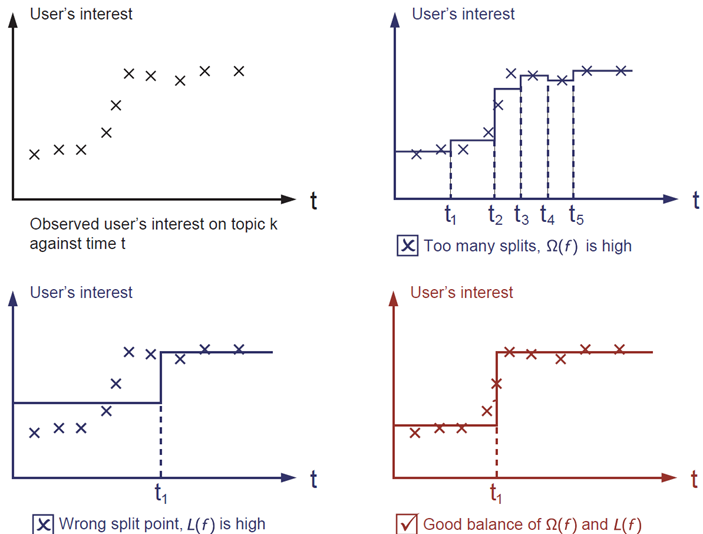
\includegraphics[width=.9\linewidth]{/home/kpapad/UG_thesis/Thesis/Dissertation/src/figures/boosted_trees_fig1.png}
\end{center}
\end{itemize}

\subsubsection{Decision Trees}
\label{sec:orgc68262f}
A decision tree is a flowchart-like tree structure, where each internal node represents a feature(or attribute), the branch represents a decision rule, and each leaf node represents the outcome.

Formally, a decision tree can be represented as a set of rules or conditions in the form of:

\texttt{f(X) = \{condition1, condition2,..condition\_n\}}

where each condition is a tuple of the form (feature, threshold, comparison operator) and the final outcome is represented by the leaf node.

For example, consider the decision tree of figure x that classify fruits based on color, shape, size, and taste. Let X be the input \texttt{X = \{"red", "smal", "sour"\}}. Then \texttt{f(X) = "grape"} 
\begin{center}
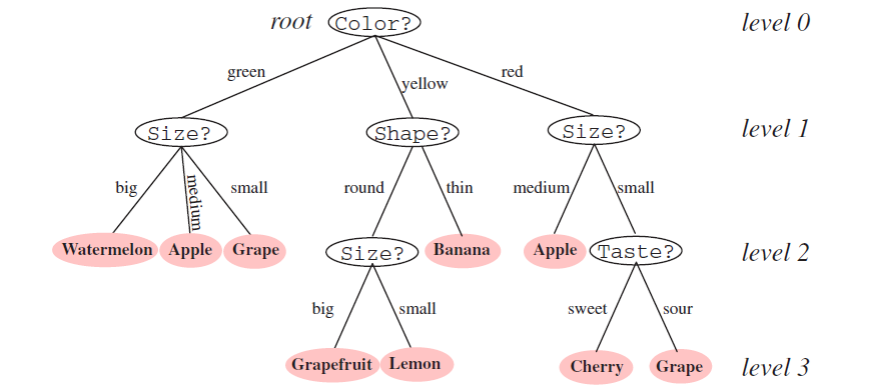
\includegraphics[width=.9\linewidth]{/home/kpapad/UG_thesis/Thesis/Dissertation/src/figures/boosted_trees_fig2.png}
\end{center} 

\begin{itemize}
\item Decision Tree Ensembles
\label{sec:org8a2fddb}

The tree ensemble model consists of a set of classification and regression trees (CART).
Let \(\mathcal{F}\) be the set of all possible CART's and \(f_{k} \in \mathcal{F}\), a function that represents a CART. The model in discussion then, can be written as:
\[
\hat{y_{i}} = \sum_{k=1}^{K} f_{k}(x_{i}),\text{ } f_{k} \in \mathcal{F}
\]

If \(\hat{y_{i}}\) represents the prediction of the tree, given an input variable \(x_{i}\), the real label of \(x_{i}\) will be denoted as \(y_{i}\)  . The objective function will be of the form:
\[
obj(\theta) = \sum_{i=1}^{n} l(y_{i}, \hat{y_{i}}) + \sum_{i=1}^{t}\omega(f_{i})
\]

where \(\omega(f_{i})\) is the complexity of a given tree  and l is the loss function.

\item Tree boosting
\label{sec:orgbee4670}

As stated earlier, the model is beeing trained, to learn those trees \(f_{k}\) that minimize the objective. The resulting model then, will be an ensemble of those functions \(f_{k}\).
The optimization of the objective, is a problem that cannot be solved with the traditional methods. Instead, the model is being iteratively trained in an additive manner.\cite{Chen_2016}
let the prediction value at the t-th iteration be \(\hat{y}^{(t)}_{i}\). In the next iteration(t+1), the chosen function \(f_{t+1}\), is such that if added to the model, the resulting prediction \(\hat{y}^{(t+1)}_{i}\) will minimize the cost function:
\[
\hat{y}^{(0)}_{i} = 0 \]
\[
\hat{y}^{(1)}_{i} =\hat{y}^{(0)}_{i} + f_{1}(x_{i}) 
\]
\[
\hat{y}^{(2)}_{i} =\hat{y}^{(1)}_{i} + f_{2}(x_{i}) 
\]

\[
\dots
\]
\[
\hat{y}_{i}^{(t)} = \hat{y}_{i}^{(t-1)} + f_{t}(x_{i})= \sum_{k=1}^{K} f_{k}(x_{i})
\]
The objective at step t is:
\[
obj^{(t)} = \sum_{i=1}^{n} l(y_{i}, \hat{y_{i}}^{(t)}) + \sum_{i=1}^{t}\omega(f_{i}) = \sum _{i=1}^{n} l(y_{i}, \hat{y}_{i}^{(t-1)} + f_{t}(x_{i})) + \omega(f_{i}(t))
\]

Taylor expanding the loss function \(l(y_{i}, \hat{y}_{i}^{(t-1)} + f_{t}(x_{i}))\), around \(f_{t}\), up to the second order and neglecting terms, referring to previous rounds, the specific objective becomes:

\[
\sum_{i=1}^{n}\left [ g_{i}f_{t}(x_{i})+\frac{1}{2}h_{i}f^{2}_{t} (x_{i}) \right ] + \omega(f_{t})
\]

Where
\[
g_{i} = \partial_{\hat{y}_{i}^{(t-1) }} l(y_{i}, \hat{y}_{i}^{(t-1)} )
\]
\[
h_{i} = \partial^{2}_{\hat{y}_{i}^{(t-1) }} l(y_{i}, \hat{y}_{i}^{(t-1)} )
\]

This is the minimization goal for \(f_{t}\) . \cite{xgboost}
\end{itemize}
